\documentclass{beamer}
\usetheme{CENIDETDIE}
\setbeamertemplate{caption}[numbered]
\usefonttheme[onlymath]{serif}

% ------------------------------------------------------------------------------------------------

\usepackage[utf8]{inputenc}
\usepackage[T1]{fontenc}
\usepackage{helvet}
\usepackage{graphicx} % Allows including images
\usepackage{booktabs} % Allows the use of \toprule, \midrule and \bottomrule in tables
\numberwithin{figure}{section}
\numberwithin{equation}{section}
\usepackage[square,sort,comma,numbers]{natbib}
\usepackage{ragged2e}
\usepackage{caption}
\usepackage{subcaption}
\usepackage{mathabx}

 

% ------------------------------------------------------------------------------------------------

\title{Work progress}
%\subtitle{Presentation in Beamer-\LaTeX}
\author{Saeed ZAHRAN $^{1,2}$  }
\institute{$^{1}$UNIVERSITÉ DE PICARDIE JULES VERNE\\ 
			$^{2}$Groupe de recherches sur l'analyse multimodale de la fonction cérébrale - INSERM}
\date{\today}

\begin{document}

% ------------------------------------------------------------------------------------------------

\begin{frame}[plain,t]
\titlepage
\end{frame}

% ------------------------------------------------------------------------------------------------



% ------------------------------------------------------------------------------------------------



% ------------------------------------------------------------------------------------------------



% ---------------------------------------------------------------------------------------
\section{}
\begin{frame}
 \frametitle{Display of MEG and OPM sensors}
 	
 	\begin{figure}[h]
        \begin{subfigure}[h]{0.4\linewidth} 
            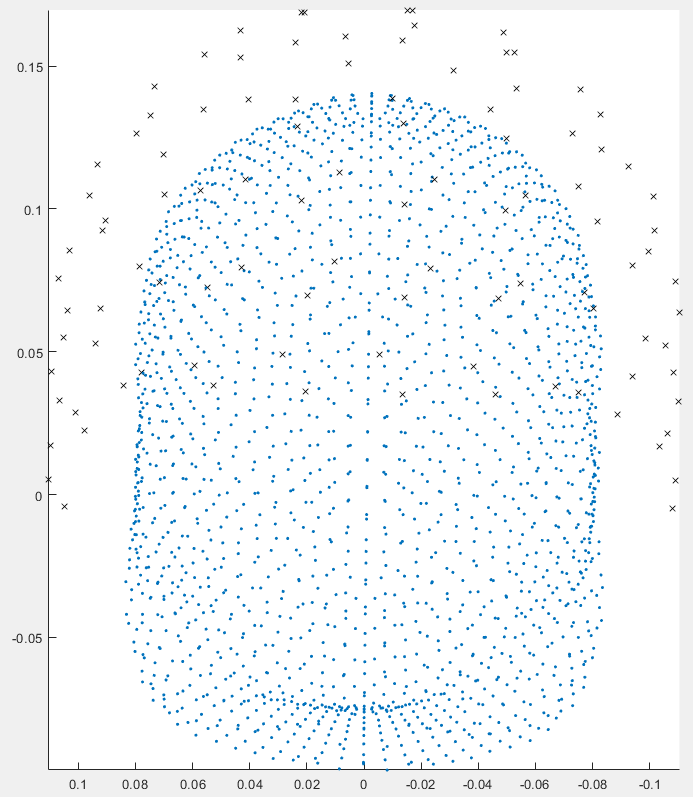
\includegraphics[width=\textwidth]{pictures/megsen}
            \caption{\scriptsize MEG sensors}
            \label{fig:rdf_graph}
        \end{subfigure}       
        \begin{subfigure}[h]{0.33\linewidth} 
            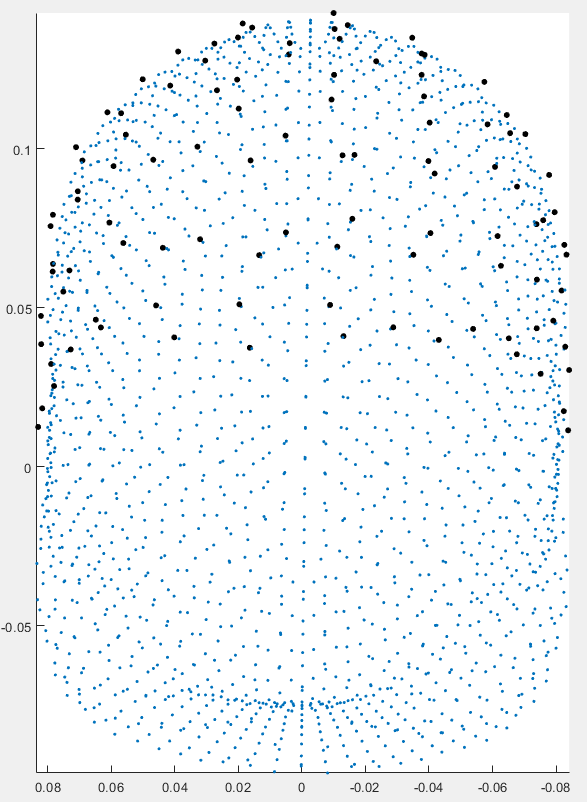
\includegraphics[width=\linewidth]{pictures/opmsen}
            \caption{\scriptsize OPM sensors}
            \label{fig:rdfs_graph}
        \end{subfigure}
       % \caption{\scriptsize Example of RDF graph and RDFS graph}
    \end{figure}
    
\end{frame}

% ------------------------------------------------------------------------------------------------
\section{}
\begin{frame}
 \frametitle{A three-dimensional OPM sensors plot displays vectors}
	\begin{figure}[p]
  		\centering
  		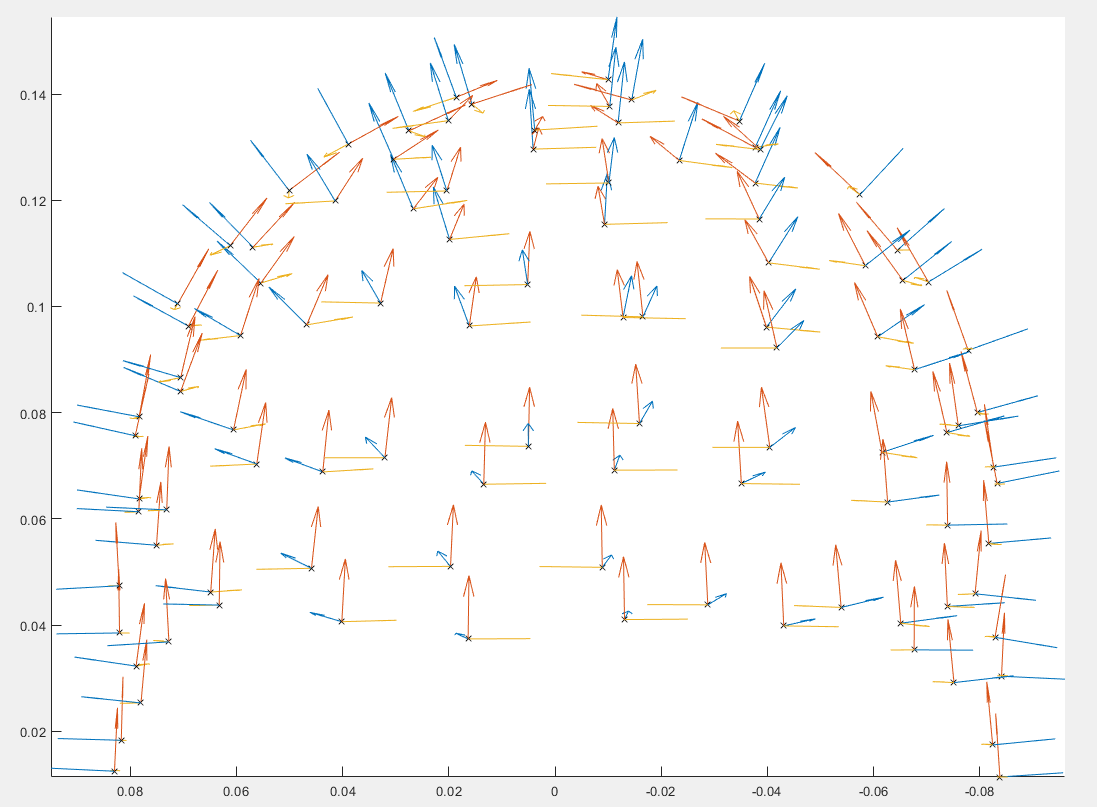
\includegraphics[width=0.6\linewidth]{pictures/opmvect}
  		%\caption{\scriptsize Main Approaches for RDF Summarization\cite{Zneika2018}}
  		\label{fig:approaches_RDF}
 	\end{figure}

  
\end{frame}

\section{}
\begin{frame}
 \frametitle{MEG - Lambda 1}
  

 	\begin{figure}[h]
        \begin{subfigure}[h]{0.53\linewidth} 
            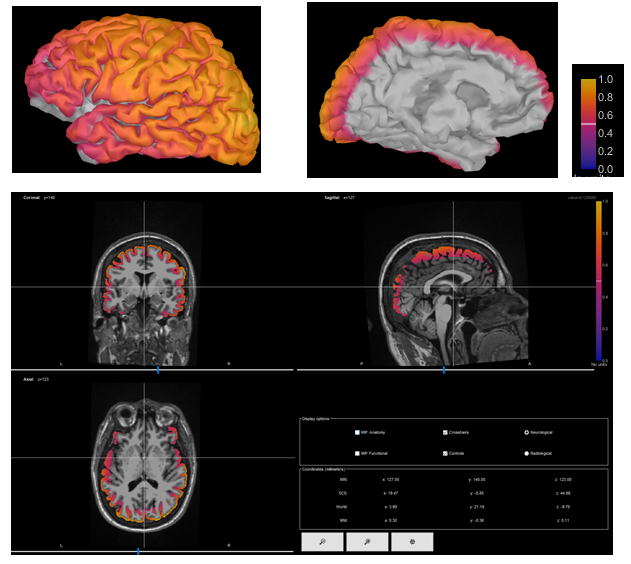
\includegraphics[width=\linewidth]{pictures/meg3}
           % \caption{\tiny RDF graph}
            \label{fig:rdf_graph}
        \end{subfigure}       
        \begin{subfigure}[h]{0.45\linewidth} 
            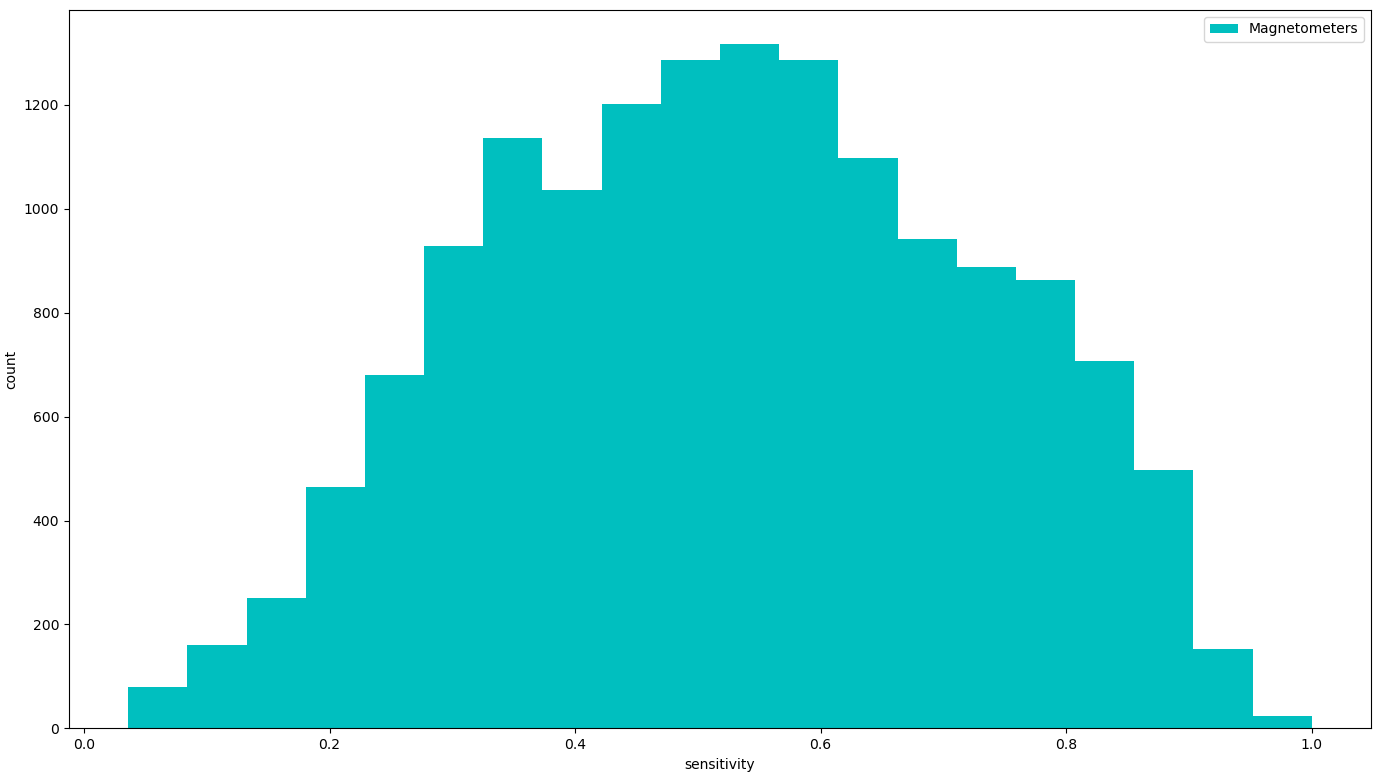
\includegraphics[width=\linewidth]{pictures/HISTmeg0.png}
           % \caption{\tiny RDF Shema (RDFS) graph}
            \label{fig:rdfs_graph}
        \end{subfigure}
       % \caption{\scriptsize Example of RDF graph and RDFS graph}
    \end{figure}

  
\end{frame}


%---------------
\section{}
\begin{frame}
 \frametitle{MEG - Lambda 2 }
  

 	\begin{figure}[h]
        \begin{subfigure}[h]{0.53\linewidth} 
            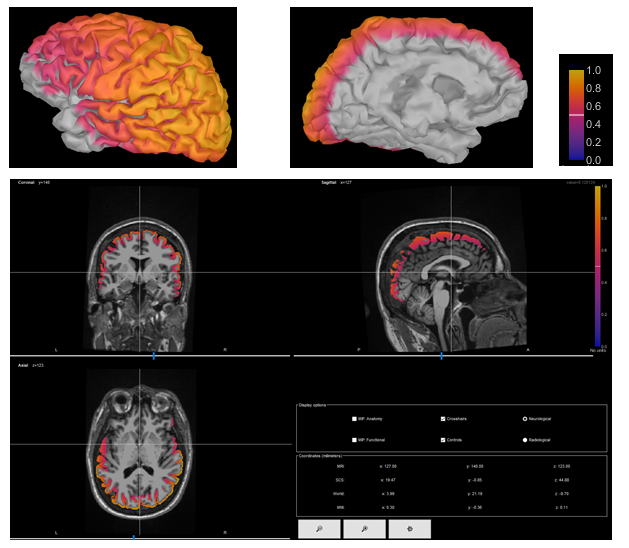
\includegraphics[width=\linewidth]{pictures/meg2}
           %  \caption{\tiny RDF graph}
            \label{fig:rdf_graph}
        \end{subfigure}       
        \begin{subfigure}[h]{0.45\linewidth} 
            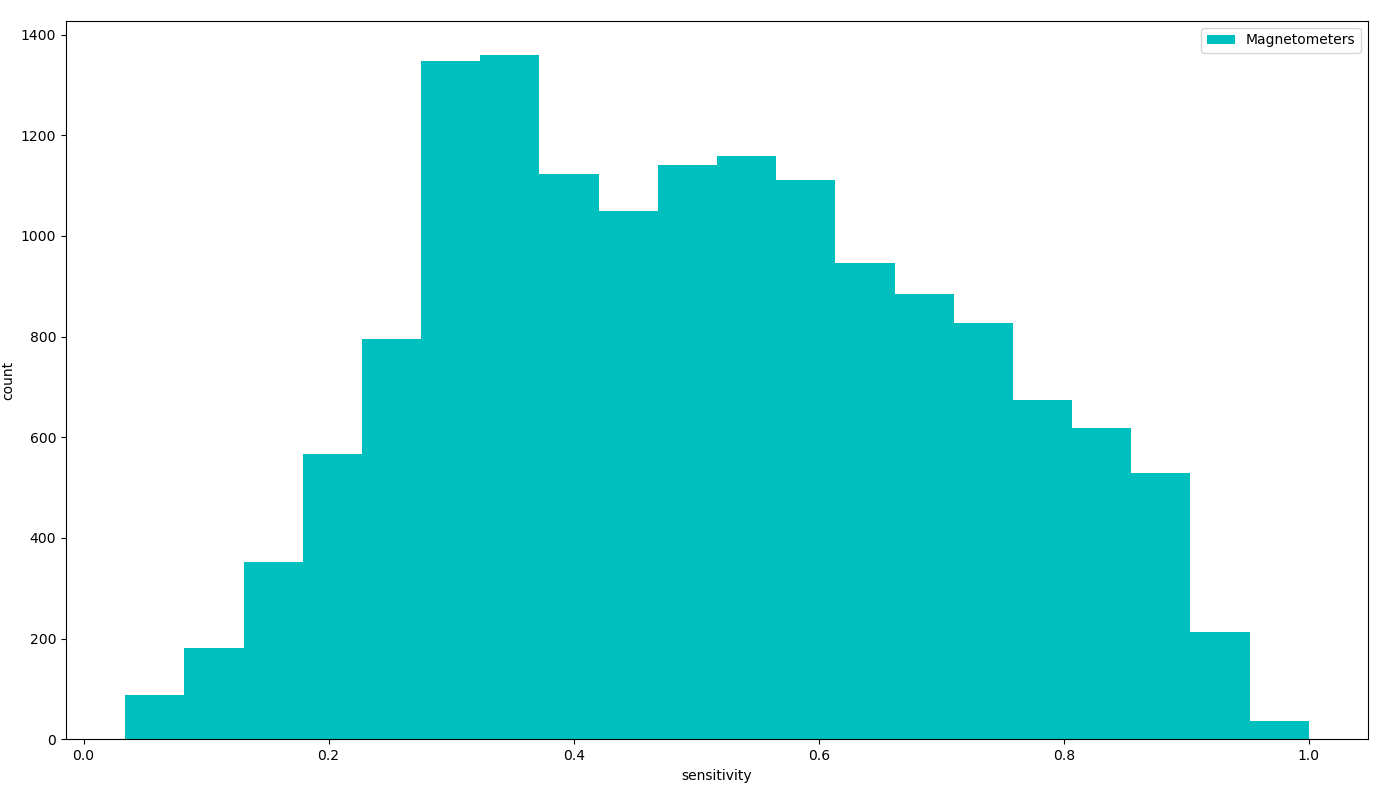
\includegraphics[width=\linewidth]{pictures/HISTmeg1.png}
             %\caption{\tiny RDF Shema (RDFS) graph}
            \label{fig:rdfs_graph}
        \end{subfigure}
       % \caption{\scriptsize Example of RDF graph and RDFS graph}
    \end{figure}

  
\end{frame}




%----------------------------------------------
\section{}
\begin{frame}
 \frametitle{MEG - Lambda min}
  

 	\begin{figure}[h]
        \begin{subfigure}[h]{0.53\linewidth} 
            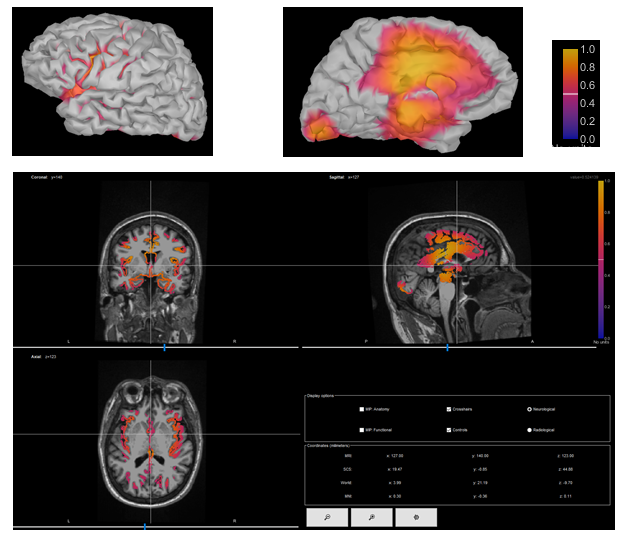
\includegraphics[width=\linewidth]{pictures/meg1}
           %  \caption{\tiny RDF graph}
            \label{fig:rdf_graph}
        \end{subfigure}       
        \begin{subfigure}[h]{0.45\linewidth} 
            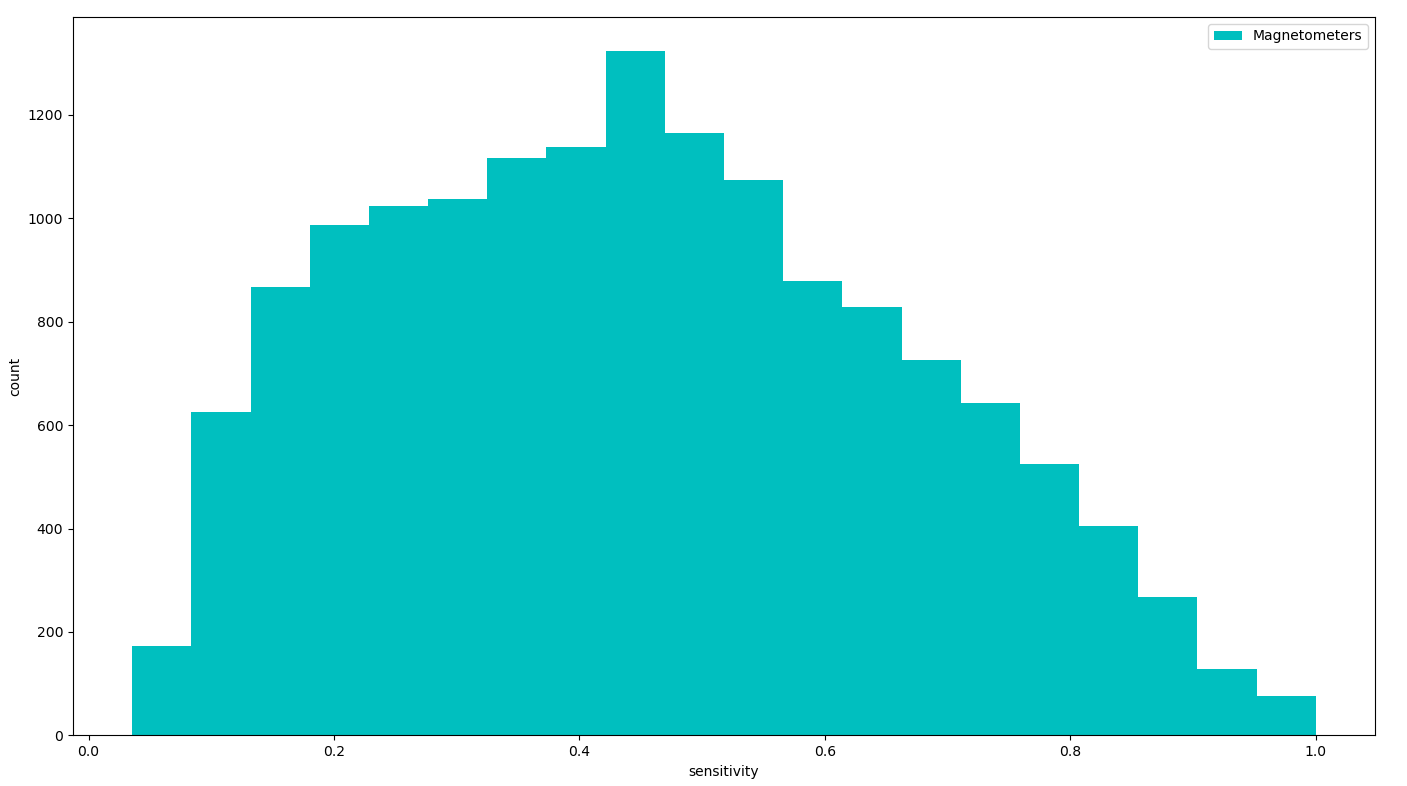
\includegraphics[width=\linewidth]{pictures/HISTmeg2.png}
           %  \caption{\tiny RDF Shema (RDFS) graph}
            \label{fig:rdfs_graph}
        \end{subfigure}
       % \caption{\scriptsize Example of RDF graph and RDFS graph}
    \end{figure}

  
\end{frame}




% ------------------------------------------------------------------------------------------------
\section{}
\begin{frame}
 \frametitle{OPMn - Lambda 1}
	\begin{figure}[p]
  		\centering
  		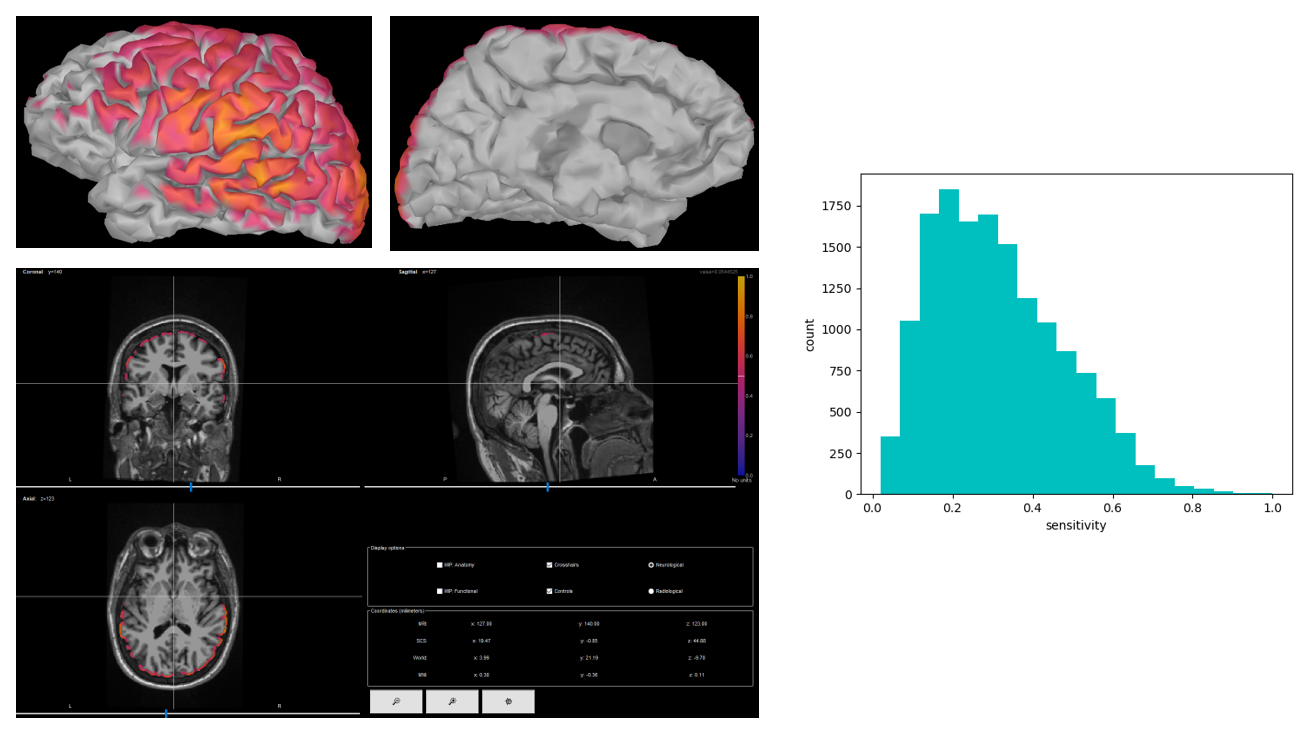
\includegraphics[width=1\linewidth]{pictures/opmsen00}
  		%\caption{\scriptsize Main Approaches for RDF Summarization\cite{Zneika2018}}
  		\label{fig:approaches_RDF}
 	\end{figure}

  
\end{frame}

% ------------------------------------------------------------------------------------------------
\section{}
\begin{frame}
 \frametitle{OPMn - Lambda 2}
	\begin{figure}[p]
  		\centering
  		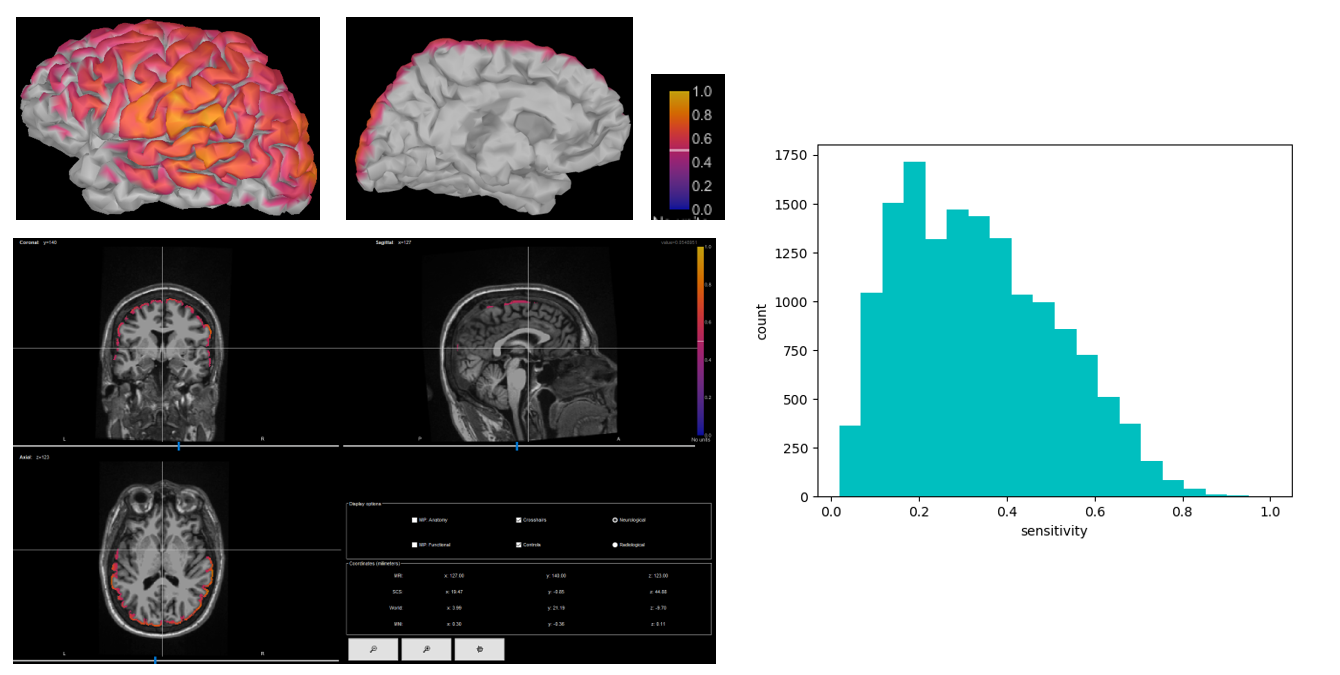
\includegraphics[width=1\linewidth]{pictures/opmsen11}
  		%\caption{\scriptsize Main Approaches for RDF Summarization\cite{Zneika2018}}
  		\label{fig:approaches_RDF}
 	\end{figure}

  
\end{frame}
% ------------------------------------------------------------------------------------------------
\section{}
\begin{frame}
 \frametitle{OPMn - Lambda min}
	\begin{figure}[p]
  		\centering
  		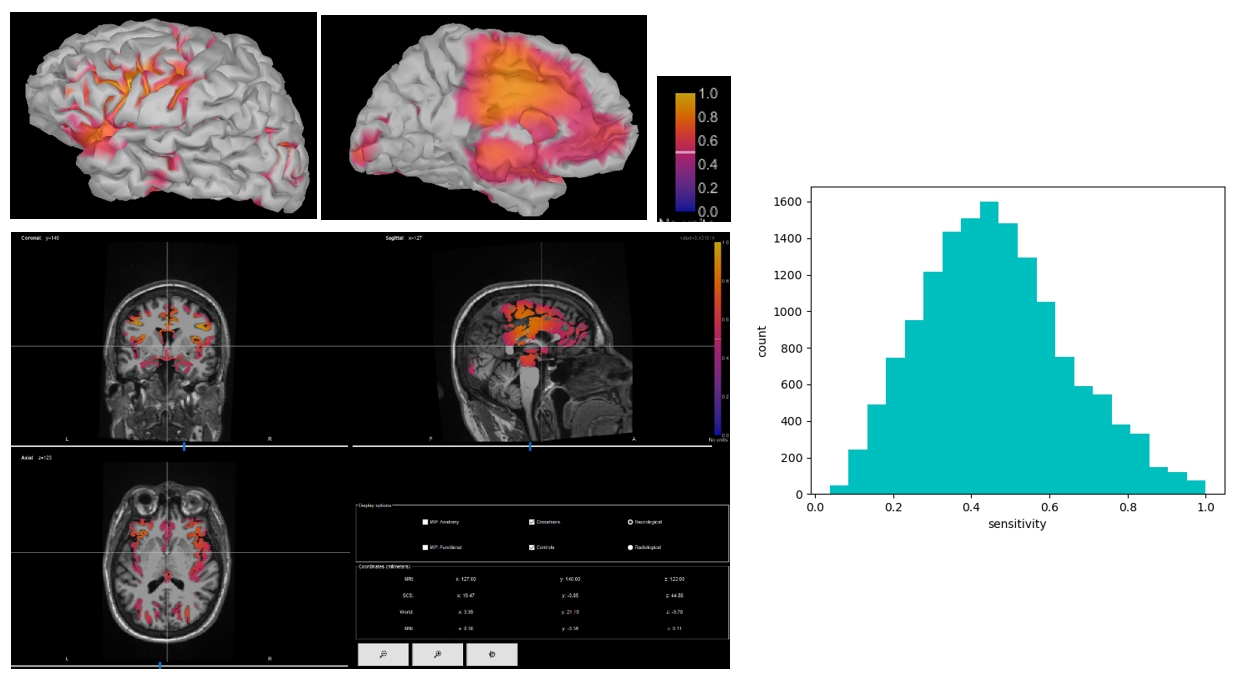
\includegraphics[width=1\linewidth]{pictures/opmsen22}
  		%\caption{\scriptsize Main Approaches for RDF Summarization\cite{Zneika2018}}
  		\label{fig:approaches_RDF}
 	\end{figure}

  
\end{frame}
% ------------------------------------------------------------------------------------------------
\section{}
\begin{frame}
 \frametitle{OPMt1 - Lambda 1}
	\begin{figure}[p]
  		\centering
  		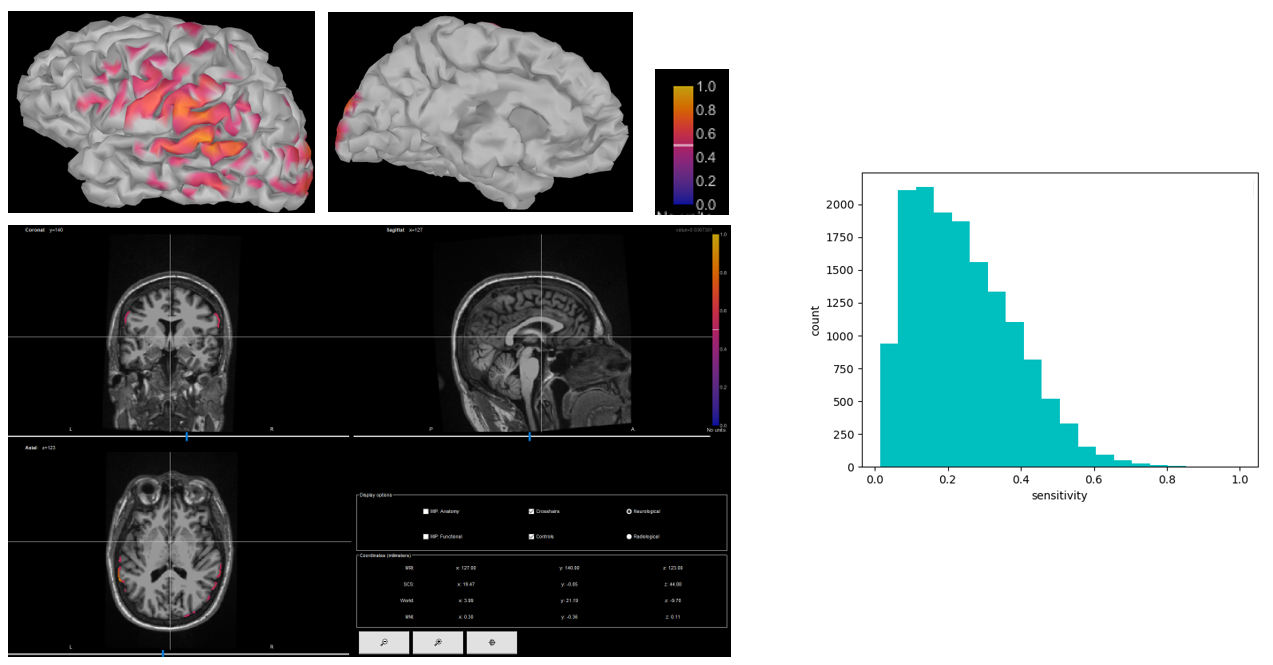
\includegraphics[width=1\linewidth]{pictures/opmt100}
  		%\caption{\scriptsize Main Approaches for RDF Summarization\cite{Zneika2018}}
  		\label{fig:approaches_RDF}
 	\end{figure}

  
\end{frame}

% ------------------------------------------------------------------------------------------------
\section{}
\begin{frame}
 \frametitle{OPMt1 - Lambda 2}
	\begin{figure}[p]
  		\centering
  		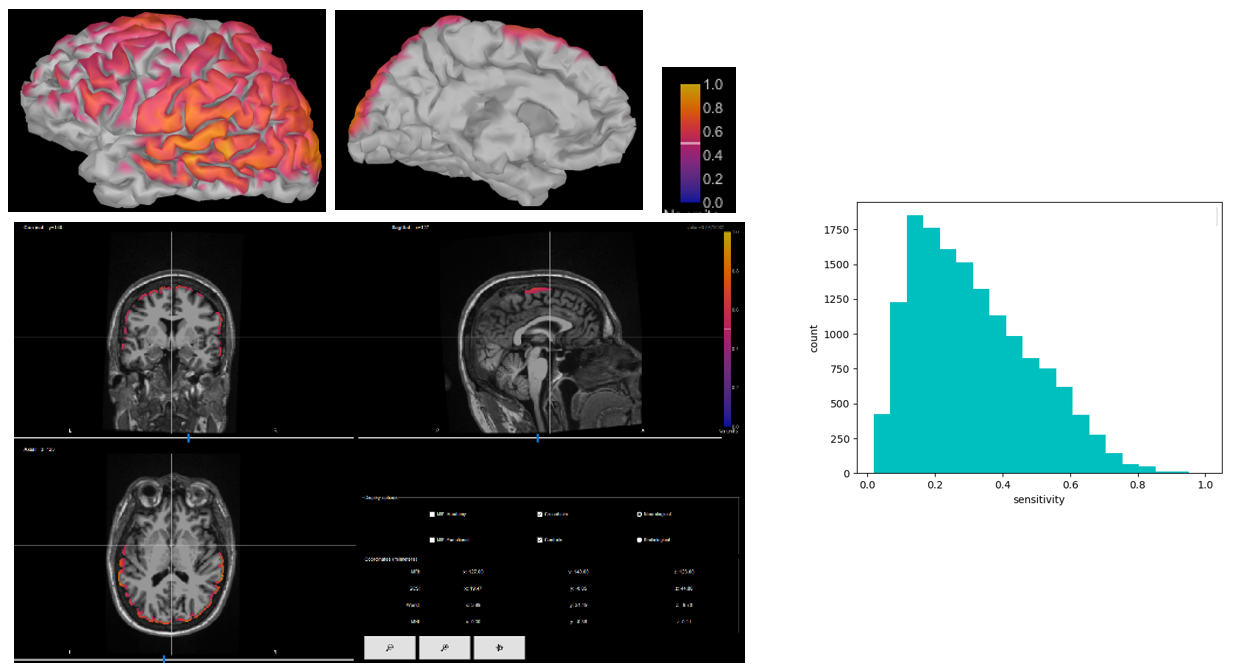
\includegraphics[width=1\linewidth]{pictures/opmt111}
  		%\caption{\scriptsize Main Approaches for RDF Summarization\cite{Zneika2018}}
  		\label{fig:approaches_RDF}
 	\end{figure}

  
\end{frame}
% ------------------------------------------------------------------------------------------------
\section{}
\begin{frame}
 \frametitle{OPMt1 - Lambda min}
	\begin{figure}[p]
  		\centering
  		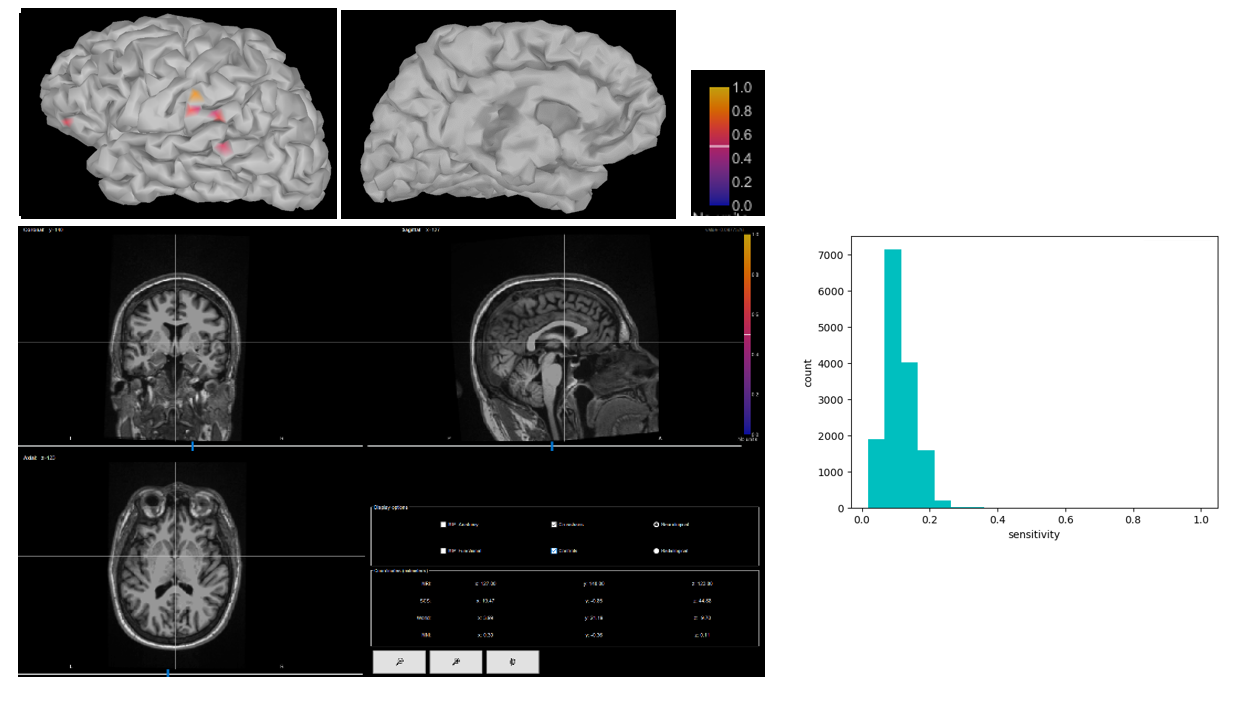
\includegraphics[width=1\linewidth]{pictures/opmt122}
  		%\caption{\scriptsize Main Approaches for RDF Summarization\cite{Zneika2018}}
  		\label{fig:approaches_RDF}
 	\end{figure}

  
\end{frame}

% ------------------------------------------------------------------------------------------------
\section{}
\begin{frame}
 \frametitle{OPMt2 - Lambda 1}
	\begin{figure}[p]
  		\centering
  		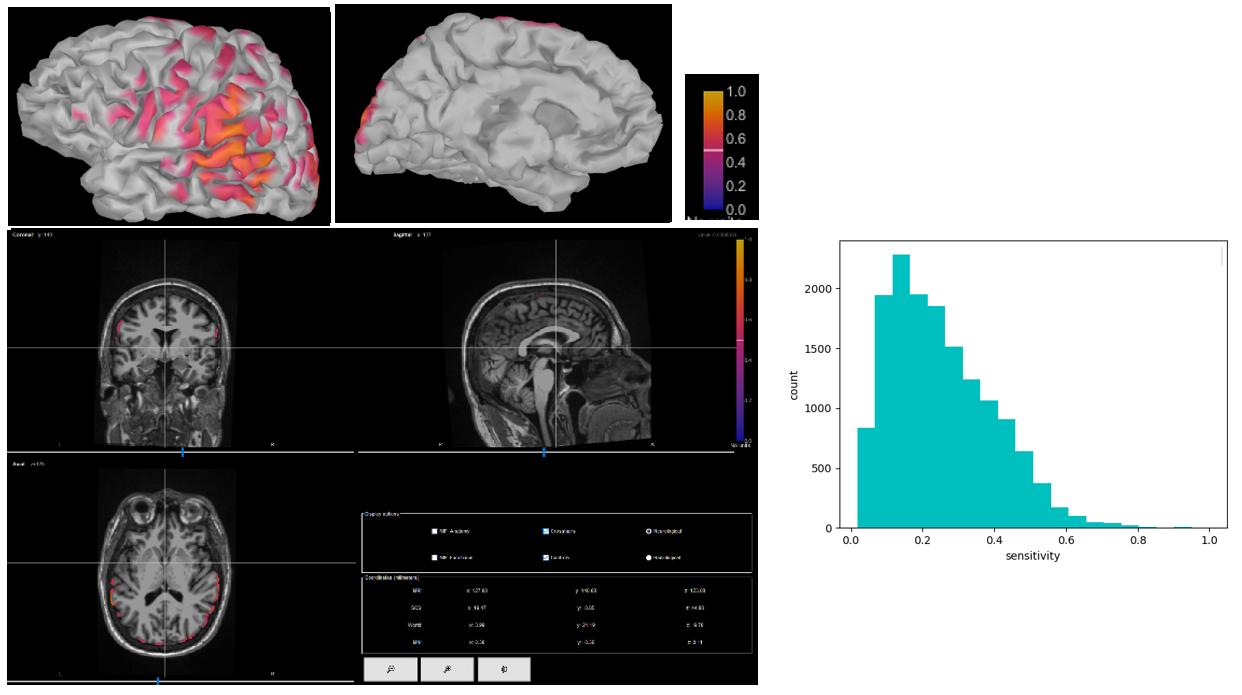
\includegraphics[width=1\linewidth]{pictures/opmt200}
  		%\caption{\scriptsize Main Approaches for RDF Summarization\cite{Zneika2018}}
  		\label{fig:approaches_RDF}
 	\end{figure}

  
\end{frame}

% ------------------------------------------------------------------------------------------------
\section{}
\begin{frame}
 \frametitle{OPMt2 - Lambda 2}
	\begin{figure}[p]
  		\centering
  		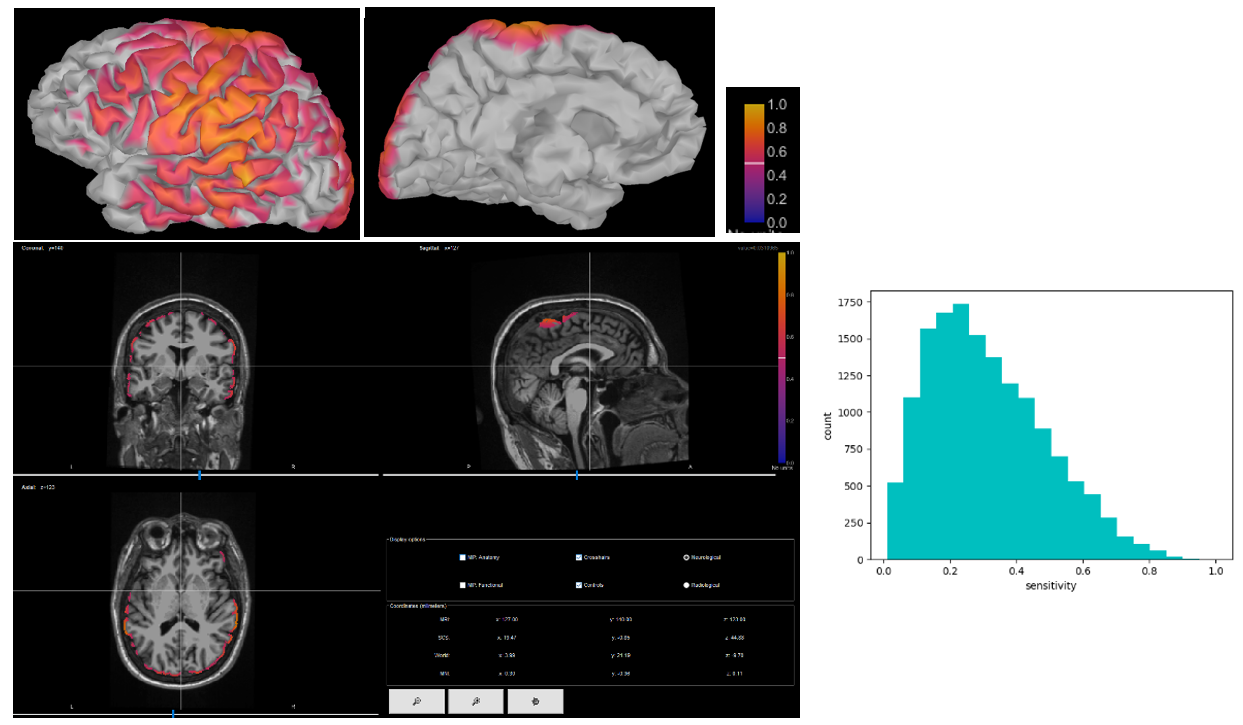
\includegraphics[width=1\linewidth]{pictures/opmt211}
  		%\caption{\scriptsize Main Approaches for RDF Summarization\cite{Zneika2018}}
  		\label{fig:approaches_RDF}
 	\end{figure}

  
\end{frame}

% ------------------------------------------------------------------------------------------------
\section{}
\begin{frame}
 \frametitle{OPMt2 - Lambda min}
	\begin{figure}[p]
  		\centering
  		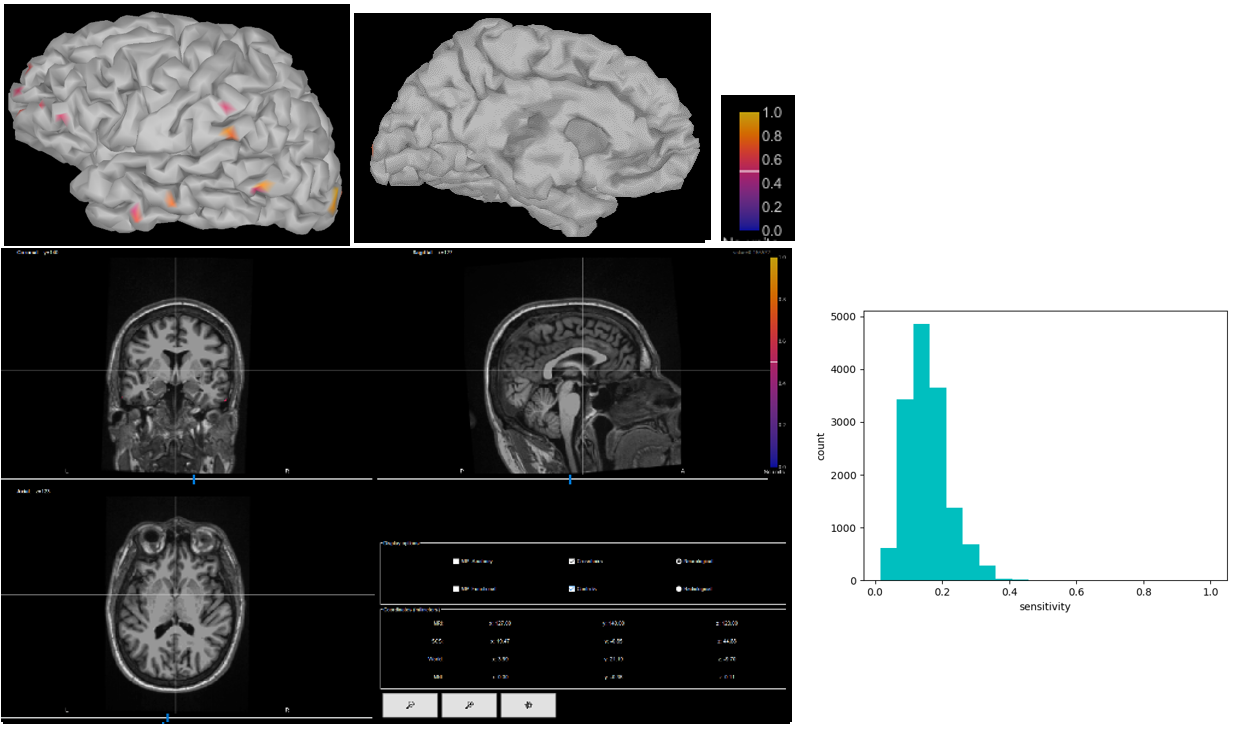
\includegraphics[width=1\linewidth]{pictures/opmt222}
  		%\caption{\scriptsize Main Approaches for RDF Summarization\cite{Zneika2018}}
  		\label{fig:approaches_RDF}
 	\end{figure}

  
\end{frame}

% ------------------------------------------------------------------------------------------------


\ThankYouFrame

% ------------------------------------------------------------------------------------------------

\end{document}
